% ----------------------------------------------------------------
% achemso --- Support for submissions to American Chemical
%  Society journals
% Maintained by Joseph Wright
% E-mail: joseph.wright@morningstar2.co.uk
% Originally developed by Mats Dahlgren
%  (c) 1996-98 by Mats Dahlgren
%  (c) 2007-2008 Joseph Wright
% Released under the LaTeX Project Public license v1.3c or later
% See http://www.latex-project.org/lppl.txt
% 
% Part of this bundle is derived from cite.sty, to which the
% following license applies:
%   Copyright (C) 1989-2003 by Donald Arseneau
%   These macros may be freely transmitted, reproduced, or
%   modified provided that this notice is left intact.
% ----------------------------------------------------------------
% 
% The achemso bundle provides a LaTeX class file and BibTeX style
% file in accordance with the requirements of the American
% Chemical Society.  The files can be used for any documents, but
% have been carefully designed and tested to be suitable for
% submission to ACS journals.
% 
% The bundle also includes the natmove package.  This package is
% loaded by achemso, and provides automatic moving of superscript
% citations after punctuation.

\documentclass[
%journal=ancac3, % for ACS Nano
%journal=acbcct, % for ACS Chem. Biol.
journal=jpcbfk, % for undefined journal
manuscript=article]{achemso}

\usepackage[version=3]{mhchem} % Formula subscripts using \ce{}
\usepackage{graphicx}
\usepackage{caption}
\usepackage{subcaption}
\usepackage[labelfont={bf}]{caption}
\usepackage{minted}

\newcommand*{\mycommand}[1]{\texttt{\emph{#1}}}

\author{Trerayapiwat K.}
\email{ktreraya@bowdoin.edu}
\affiliation[Bowdoin College]
{Department of Chemistry, Bowdoin College, Brunswick, ME}
\author{Eustis S.}
\email{seustis@bowdoin.edu}
\affiliation[Bowdoin College]
{Department of Chemistry, Bowdoin College, Brunswick, ME}


\title[\texttt{achemso} demonstration]
{Benchmarking Ab Initio Computational Methods for the Quantitative Prediction of Sunlight-Driven Pollutant Degradation in Aquatic Environments}

\begin{document}


\begin{abstract}
Understanding excitation from ground state to the singlet excited state through simulating absorption spectra of a molecule is essential to predicting the rate of the photoreaction. Excitation energies and oscillator strengths were calculated using different theories and methods. Among all theories, a new approach was selected to model the photon absorption: Molecular Dynamics–Time Dependent Density Functional Theory (MD-TDDFT). An aniline molecule equilibrates in the presence of a number of water molecules at room temperature using 6-311++G** basis set. Excitation energy and oscillator strength of aniline geometries in equilibrium are then calculated using TDDFT with w-B97X-D, CAMB3LYP, or M06-2X functional. As a theoretical benchmark, OEMCCSD calculation was carried out with optimized geometry from using using 6-311++G** basis set and implicit water model implemented using Polarizable Continuum Model (PCM). The computed physical properties from MD-TDDFT and OEMCCSD were then compared with data from experimental absorption spectra to evaluate the accuracy of the two methods. Absorption spectra’s underlying modified Gaussian functions were decomposed and integrated to calculate experimental oscillator strength at a certain excitation energy using an R code written by Peter Cohen. The more accurate method would be applied to triclosan and other water contaminants to predict the rate of their photodegradations in the environment.
\end{abstract}


\section{Introduction}

\subsection{Environmental Photochemistry And Micropollutants}

During the past century, more and more synthetic chemicals has been created for commercial pharmaceuticals and personal care products. Many have found their way back into the environment predominantly into water. Each year, about 300 million tons of organic chemicals are being added into water systems.\cite{Schwarzenbach2006} These chemicals has been detected in ng/L to μg/L in the aquatic systems worldwide.\cite{Monteiro2010} The scale of chemicals being introduced into the water reaffirms the need for close studies in order to understand the consequences of these compounds on the environmental system, and eventually to living beings. While major toxic chemicals, such as \ce{CCl4}, DDT etc., has been constantly regulated or banned by governments for its effects on agriculture and the environment, many more compounds have not received the attention they deserve. Even though some are approved as safe for daily usage in household products, their impacts after being disposed into water  remains largely unknown. These low-concentration chemicals are collectively called mictopollutants. Study of a particular micropollutant is hard to conduct because other species often interfere in analytical reactions. Triclosan, a micropollutant, has been used as an anti-bacterial agent in household soap and health care products. Under sunlight, Triclosan decomposes to Dioxins and PCBs, well-known carcinogens.\cite{Bedoux2012} Previously, computational studies of Triclosan in the excited states were carried out by Soren N. Eustis.\cite{Kliegman2013}  

\subsection{Environmental Photochemistry And Micropollutants}

While excited states are important to understanding photochemical reaction, excitation from ground states by photons to exited states is equally important to understand complete reaction mechanism. There are currently no studies on quantitative calculation of excited state energies of organic molecule in water. This allows room for a systematic approach to develop a computational model and . After calculation of excited state energies and the oscillator strength, computational results will be compared with experimental UV-VIS spectrum to evaluate accuracy of the models used. 

Nathan Ricke.\cite{Ricke2014}

\subsection{Solvent Models}

Despite recent advent of growth in computer speed and burgeoning interest in incorporating computational models to further understand the nature world, large systems such as solvation models remains a big challenge.\cite{Lin2007} In modeling effects of solvent molecules on solute, implicit solvation models were previously implemented because it allows for acceptable results calculation while maintaining good speed (low computational cost). Most famous of all implicit models is Potential Continuum Model (PCM).\cite{Cossi2000} Instead of explicitly handling each solvent molecules quantum mechanically, PCM expresses their bulk effects on solute molecule in means of dielectric continuum field surrounding molecule of interest. Its downfall is that, however, its accuracy falls short of static and dynamic contribution of excited states properties.\cite{Barone2007} Furthermore, implicit solvent model also neglects hydrogen-bonding as it assumes implicit implementation in dispersion forces and electrostatics.\cite{Li1999} Especially in calculating excited state energies, an accurate solvent model should be used.\cite{Tomasi2005} In explicit solvent model, one recent notable method – Effective Fragment Potentials (EFP) can be used to model explicit solvents with non-bonded van der Waals interactions, hydrogen bonding using Coulomb interactions, polarization, and exchange repulsion without high computational expense of explicit models.\cite{Day1996,Yoo2008} This model is chosen to implement explicit solvent in calculating excited states energies.

In modeling organic solute in aquatic environment, the solute, the appropriate number of water molecules to be included as EFP in the model has never been evaluated. Too many water means expensive computational cost. Too few water will not fully model solvating shells around the solute. Binary system will be used to model how many water molecule is needed to fully solvate the solute molecules: 2, 4, 8, 16... Once excited energies for each system is calculated, the results will be compared with experimental value to evaluate how many water is needed before determining on which functional out of three choices should be chosen to achieve the most accurate computational model. 


\section{Method}

\subsection{Computational Models: Theories, Basis Sets, and Functionals}

Among all current theories, Time-Dependent Density Functional Theory (TDDFT) is the most promising with its high accuracy when used with appropriate functionals and low computational cost\cite{Magyar2007}. Implementing EFP solvent model, TDDFT can be used to accurately calculate excited state energy of acetone in water.\cite{Yoo2008} Typically in Implicit solvent model, geometry optimization of solute molecule is carried out with PCM, followed by calculation of excited state energies, also with PCM. This static ground state molecule however does not accurately represent solute in water.\cite{Defusco2011} Instead, Molecular Dynamics (MD) of solute and solvent fragments can be used to obtain a range of equilibrated structures for excited state energies calculation. Mark Gordon averaged the calculated energies of each excited state to arrive at a final excited states energy.\cite{Defusco2011} 

According to previous basis set studies, wile having roughly the same computational cost, an average-sized basis set 6-311++(2d,p) performs better than aug-cc-pVDZ (ACCD).\cite{Wiberg2004,Barnes2014} For example, transition energies calculated of CN molecule as calculated by ACCD deviates 1117-1669 cm\textsuperscript{-1} from experimental value while those by 6-311++(2d,p) only deviate 220-470 cm\textsuperscript{-1}. Hoping to most accurately calculate the excited energies, 6-311++(2d,p) basis set is chosen to run TDDFT after MD run. In running MD, a smaller basis set 6-31+(2d,p) will be used in order to cut computational cost. The decision comes after weeks of waiting for computational results when determining the number of water molecule in the model. Two best-performing DFT functionals out of all examined in previous study are explored: CAMB3LYP, M06-2X.\cite{Barnes2014} PBE0 will also be used.

Molecules - aniline - then para-methoxy m-methoxyacetophenone... Triclosan

discuss \# of water



\section{Preliminary Results and Discussions}

\subsection{Determining the number of water}

TDDFT calculation for aniline with 32, 64, 128, 256, 512 surrounding water molecules were performed with CAMB3LYP basis set. Firstly, for 32 water molecules, the equilibrium were chosen to start from 15 ps and the stopping point of calculation was 25 ps; 1000 jobs for every 10 fs. Determination of equilibrium was determined by eyeballing a plot of the solvent solute system's potential energy over time for a stable period as shown in the figure \ref{fig:MDEnergyAniline32d)}. The consistently low fluctuation indicates the start of equilibrium at 15000 fs. 1000 frames or 10000 fs of MD geometries were used to calculate the excitation energies in TDDFT run. Geometry of the system though challenge the accuracy of 32-water model. Aniline molecule surrounded in 32 water molecules is unfortunately most stable not being fully solvated. Aniline can be seen outside of the water cluster at the time of equilibrium. This is in contrast to expected 32 water as the first solvation shell for aniline. \cite{Plugatyr2009} 

\begin{figure}[!tbp]
	\centering
		 \begin{subfigure}[b]{0.4\textwidth}
		 	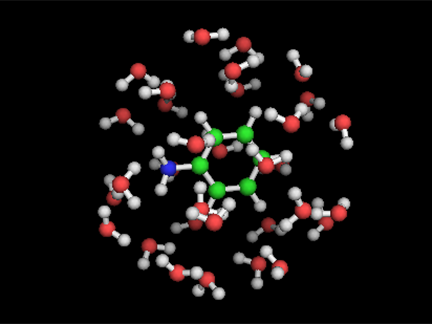
\includegraphics[width=1\textwidth]{CAMB3LYP/aniline32_0fs.png}
		 	\caption{}
		 	\label{fig:MDEnergyAniline32a)}
		 \end{subfigure}
		 \hfill
		 \begin{subfigure}[b]{0.4\textwidth}
		 	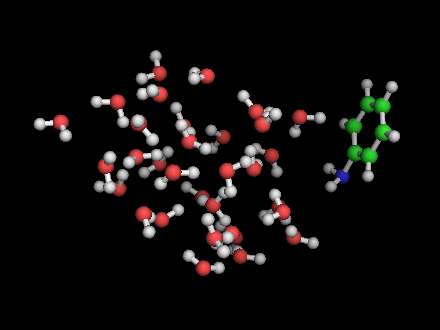
\includegraphics[width=1\textwidth]{CAMB3LYP/aniline32_15000fs.png}
		 	\caption{}
		 	\label{fig:MDEnergyAniline32b)}
		 \end{subfigure}
		 \hfill
		 \begin{subfigure}[b]{0.4\textwidth}
		 	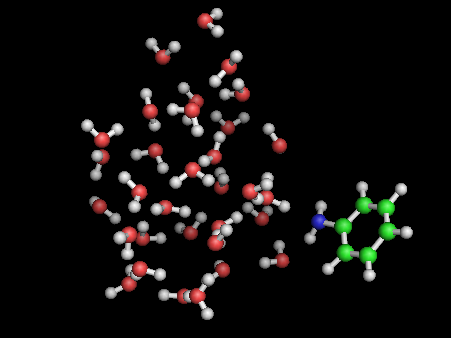
\includegraphics[width=1\textwidth]{CAMB3LYP/aniline32_25000fs.png}
		 	\caption{}
		 	\label{fig:MDEnergyAniline32c)}
		 \end{subfigure}
		 \hfill
		 \begin{subfigure}[b]{0.4\textwidth}
		 	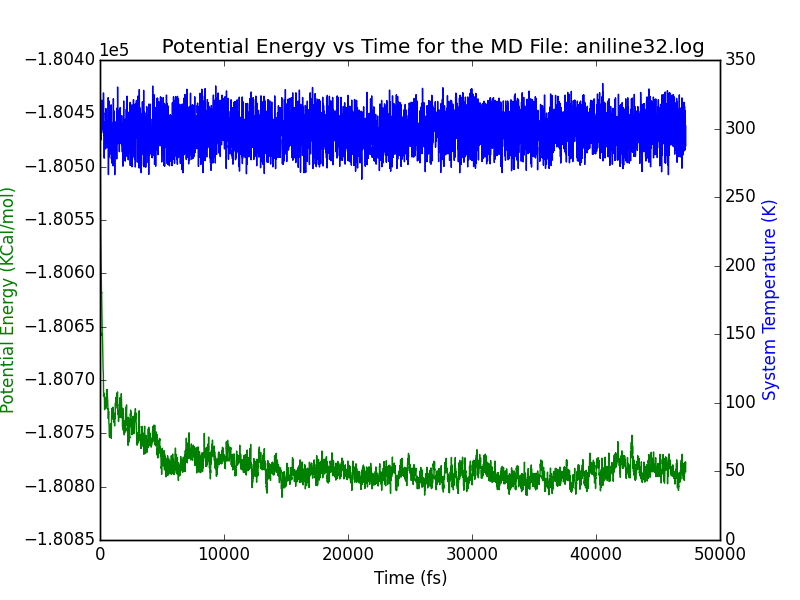
\includegraphics[width=1\textwidth]{CAMB3LYP/aniline32_EnergyPlot.png}
		 	\caption{}
		 	\label{fig:MDEnergyAniline32d)}
		 \end{subfigure}
	\caption{Molecular Dynamics run of aniline in 32 explicit solvating water molecules. Notice that at equilibrium, aniline molecule comes outside of the water sphere. Albeit hydrogen bond being clearly established, lack of total submersion in water means 32-water does not fully solvate the aniline molecule and suggests that 64-water will give more accurate results. (a) starting geometry of MD run created by packmol. (b) geometry after 15000 fs. Notice the hydrogen bond between the amino group and water cluster. (c) geometry after 25000 fs. The amino group is pointing in the water sphere, as it continues to through out the whole MD run. (d) A plot of potential Energy of the system vs time. At 15000 fs, equilibrium starts as evident by decrease in energy fluctuation.}
	\label{fig:MDEnergyAniline32}
\end{figure}

%for refing page number
%function grows near 0. Also, in the page \pageref{fig:mesh1}

\begin{table}[ht]
	\caption{Wavelength and Oscillator Strength from MD-TDDFT calculation of aniline in 32 water molecules.}
	\label{table:aniline32TDDFTTable}
	\centering
	\begin{tabular}{c c}
		Wavelength (nm) & Oscillator Strength\\ [1ex] % inserts table %heading
		\hline\hline
		\\[-0.5ex]
		173.00&0.165685\\
		180.20&0.364739 \\
		184.99&0.339029\\
		214.30&0.143915\\
		246.26&0.0383513\\ [1ex]
	\end{tabular}
\end{table}

The excited state energies and its oscillator strength are tabulated in table \ref{table:aniline32TDDFTTable}. When compared with aniline's UVVIS spectra, as in figure \ref{fig:UVFromR}, there are several problems. Firstly, the calculated value at 246 nm does not appropriately capture  the peak at 230 nm and there is no calculated excitation energy at 280 nm, where the experimental peak is. The problem is probably due to aniline not being fully solvated. 



\begin{figure}[htb]
	\centering		
	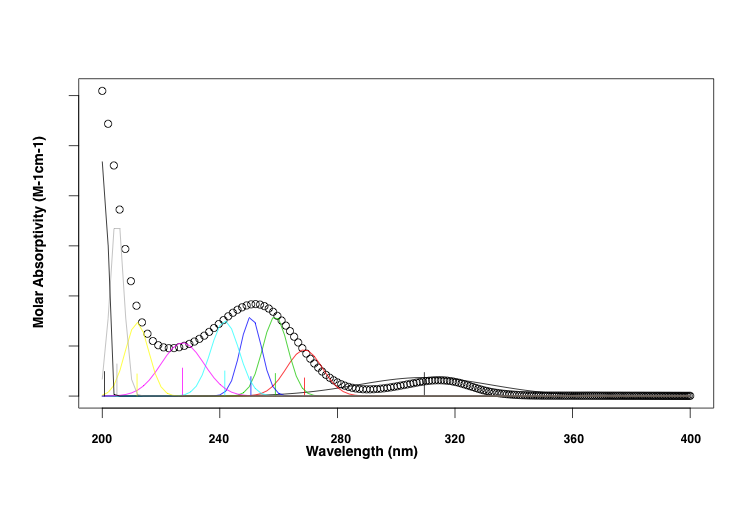
\includegraphics[width=1\textwidth]{UVVISFromR.png}
	\caption{Experimental UVVIS spectra. Gaussian plots are fitted under the curve to find oscillator strength underlying the curve. Note here that data starts from 200 nm to 400 nm. Wavelength oscillator strength of underlying gaussians are reported in table.}
	\label{fig:UVFromR}
\end{figure}

\begin{table}[ht]
	\caption{Wavelength and Oscillator Strength calculated from experimental UV-VIS spectrum using Bayesian probability (see appendix for R code).}
	\label{table:anilineUVTable}
	\centering
	\begin{tabular}{c c}
		Wavelength (nm) & Oscillator Strength\\ [1ex] % inserts table %heading
		\hline\hline
		\\[-0.5ex]
		241.53&1808.0\\ 
		234.52&2251.3\\
		228.95&1939.4\\
		223.28&2506.5\\ 
		214.67&2795.1\\
		206.10&2208.4\\
		202.53&3202.8\\
		200.39&2447.5\\[1ex]
	\end{tabular}
\end{table}

\clearpage
\appendix 
\label{appendix}
\section*{Appendix}
\renewcommand{\thesubsection}{\Alph{sub}}
	\subsection{Python Scripts}
	In order to automatically generate input files and cultivate output data from output files, many python scripts are written from scratch. Since scripts are specific to each GAMESS run, there is a limited number of scripts available on the internet (virtually none for this project). Log files obtained from GAMESS contains both valuable experimental data and useless text strings. Python scripts play an important role in both data collection and smoothing up the process between each computational steps.  For example, even though WEBMO can generate sets of latest geometry in MD run, but retrieving geometry from each MD step requires one to manually open the log file and copy-paste the geometry into input files of the next step one by one. The python script postMDDataPull2.py is designed to pull thousands of geometries and generate GAMESS input files for TDDFT energy calculation within seconds. Generating these python scripts will also allow unified program to be developed in order to automate the whole project without any manual input.

		\subsubsection{Preparing MD Input Files}
			This script does two things. First (line 35-84), it calculates appropriate radius for solvent boundary potential. Some time and effort were spent on figuring out what the radius should be without emperically guess it. A simple model is proposed: At most solute will rotate around its outmost solute atom. This radius, in the code, is called solute radius. The other radius is solvent radius, its the distance between the outmost solvent atom to the solute's CG. These two radius plus an extra 2-3 Angstrom gives ssbp radius for MD input file. Second (line 87-155), the script parses xyz file's geometry data into MD input file. Slight format change is required for GAMESS input files, so this python code automate that change. The output file is MD file which can be run on GAMESS. Output of this script can be seen below in MD Input File section.
			\vfill
			\inputminted[linenos, breaklines, baselinestretch=1, fontsize=\small]{python}{../pythonScripts/prepareMD2.py}
		
		\subsubsection{MD Geometries extraction}
			One of the reasons, an MD run might fail is if solute molecule is pushed out of the water sphere. 3dExtract4.py allows geometries to be extracted into a xyz-movie file. xyz files, capable of containing more than one frame of geometries, allows one to follow MD through a combination of screenshot (each frame is 10 femtosecond - in the current MD input file - see MD Input File section). 
			\inputminted[linenos, breaklines, baselinestretch=1, fontsize=\small]{python}{../pythonScripts/3dExtract4.py}
			
		\subsubsection{Plot Potential Energy of MD run}
			plotEnergyMD6.py script is used to extract potential energy and temperature of each MD frame to determine the if the system has equilibrated. This and 3dExtract are very essential to the first stage of the project: they determine whether MD has failed or reached equilibrium based on the geometry and potential energy of the system. Many versions of this code has been developed and this is the most refined piece of code for its purpose. Future work can be done on plotting the plot on Matlab instead of obviously inferior python counterpart - matplotlib. 
			\inputminted[linenos, breaklines, baselinestretch=1, fontsize=\small]{python}{../pythonScripts/plotEnergyMD6.py} 	
		
		\subsubsection{Find The Most Equilibrated Period}
			There are currently no consensus as to when MD has reached the equilibrium. In the past, plotEnergyMD (previous script) was used to indicate whether the potential energy of the system(solute and solvent) has stabilized. Arbitrariness in deciding whether the equilibrium is reached falls in the hands of users. findEquilibrium.py is designed to solve this subjectivity. With a list of potential energies at different time from plotEnergyMD, linear fit can be done in a fix interval to evaluate the rise or fall in energy. Currently, the limit value is taken, still empirically, from 15000 to 25000 fs interval in CAMB3LYP aniline32.log. Further improvement can be done to find the bottom slope limit as a variable with molecule input.
			\inputminted[linenos, breaklines, baselinestretch=1, fontsize=\small]{python}{../pythonScripts/findEquilibrium.py} 
		
		\subsubsection{Prepare TDDFT input}
			After equilibrium is determined, fincut2.py can be used to create TDDFT input files from xyz-movie file. a Text file containing gmssub commands especially for Bowdoin hpc grid is created. The script was created by Nathan Ricke for this work, but many improvement has been made. The new script works faster and more efficient, even though it still has outdated syntax and methods.
			\inputminted[linenos, breaklines, baselinestretch=1, fontsize=\small]{python}{../pythonScripts/fincut2.py} 
		
		\subsubsection{Pull Excited State Energies from TDDFT Log Files}
			postMDDataPull2.py pulls out excited state energies and dipole moments. Energy output is in the format of time, S1, S2... Dipole output is in the format of time, X1, Y1, Z1, X2...
			\inputminted[linenos, breaklines, baselinestretch=1, fontsize=\small]{python}{../pythonScripts/postMDDataPull2.py} 
		
	\subsection{GAMESS inputs}
		\subsubsection{MD Input File}
			 MD run is core to modeling explicit solvent. The MD run is simulated every femtosecond but only record every 10 femtoseconds. The bath temperature is 25 $\pm$ 25 degree Celsius. Solvent boundary potential is also actiavetd using default Sforce value, but with estimate ssbp radius. \#\#\#\#\#\#\#\#\#n\#\#\#\#\#\#\#\#\# are for restarting MD in case the calculation abruptly ends (see next section). In this version, dispersion correction is not turned on. Basis set = 6-31+(2d,p)
			 \inputminted[linenos, breaklines, baselinestretch=1, fontsize=\small]{Perl}{../GAMESSinpSample/MD_aniline32.inp}
			 
		\subsubsection{MD Restart}
		\#\#\#\#\#\#\#\#\#n\#\#\#\#\#\#\#\#\# are for restarting MD. For example, if MD stops from errors at t= 39000 fs, a restart geometry and \$MD should be obtained from t= 38960 in the run's trj file. \#\#\#\#\#\#\#\#\#1\#\#\#\#\#\#\#\#\# from trj goes to \#\#\#\#\#\#\#\#\#1\#\#\#\#\#\#\#\#\# in MD input file and so on with 2 and 3.
		\inputminted[linenos, breaklines, baselinestretch=1, fontsize=\small]{Perl}{../GAMESSinpSample/MD_aniline32.trj}
		
		\subsubsection{TDDFT Input File}
			Excited state energies are calculated using TDDFT. Direct SCF calculation is turned on. Basis set = 6-311++(2d,p)
			\inputminted[linenos, breaklines, baselinestretch=1, fontsize=\small]{Perl}{../GAMESSinpSample/TDDFT_aniline32_15010.inp}


\acknowledgement

Sed aliquam euismod nunc nec consectetur. Fusce eget dui id tortor tristique luctus. Pellentesque elit eros, molestie et molestie vitae, laoreet in risus. Nullam ligula lectus, pulvinar eget sagittis sed, cursus ac magna. \ldots


\suppinfo

Ut volutpat, felis sit amet malesuada blandit, arcu sapien feugiat libero, vel interdum ipsum dolor et dolor. Fusce tortor sapien, pharetra sit amet posuere ac, viverra mollis est. Maecenas auctor ultrices quam a pharetra. Aenean ornare dictum libero vitae gravida. Mauris auctor sapien at purus accumsan lacinia.

\bibliography{citation.bib}

\end{document}
